% ANUfinalexam.tex (Version 2.0)
% ===============================================================================
% Australian National University Final Exam LaTeX template.
% 2004; 2009, Timothy Kam, ANU School of Economics
% Licence type: Free as defined in the GNU General Public Licence: http://www.gnu.org/licenses/gpl.html

\documentclass[a4paper,12pt,fleqn]{article}
\setlength{\parindent}{0em}
\usepackage{amsmath}
\usepackage{fancyhdr}
\usepackage{siunitx}
\usepackage{enumitem}
\usepackage{amsmath}
\usepackage{graphicx}
\usepackage{tikz}
\usepackage{import}
\usepackage{comment}

% Unit definitions %%%%%%%%%%%%%%%%%%%%%%%%%%%%%%%%%%

\DeclareSIUnit\kilowatthour{kWh}
\DeclareSIUnit\kilowattpeak{kW_P}
\DeclareSIUnit\kVA{kVA}
\DeclareSIUnit\kVAR{kVAR}
\DeclareSIUnit\year{y}
\DeclareSIUnit\north{N}
\DeclareSIUnit\south{S}


% Insert your course information here %%%%%%%%%%%%%%%%%%%%%%%%%%%%%%%%%%

\newcommand{\institution}{CORNWALL COLLEGE}
\newcommand{\titlehd}{BSc Renewable Energy and Carbon Management}
\newcommand{\examtype}{Referral Assignment}
\newcommand{\examdate}{Academic Year 2014-2015}
\newcommand{\examcode}{CORC2100}
\newcommand{\examtitle}{Sustainable Energy Management}
\newcommand{\readtime}{15 Minutes}
\newcommand{\duedate}{Thursday $20^{\mathrm{th}}$ August}
%\newcommand{\materials}{Non-programmable Calculators; Formula Sheet}
\newcommand{\submission}{Please submit to the Assessment Moodle site by the due date}
\newcommand{\middlewords}{Assignment continues on next page}
\newcommand{\lastwords}{End of Assignment}

%%%%%%%%%%%%%%%%%%%%%%%%%%%%%%%%%%%%%%%%%%%%%%%%%%%%

%\setcounter{MaxMatrixCols}{10}
\newtheorem{theorem}{Theorem}
\newtheorem{acknowledgement}[theorem]{Acknowledgement}
\newtheorem{algorithm}[theorem]{Algorithm}
\newtheorem{axiom}[theorem]{Axiom}
\newtheorem{case}[theorem]{Case}
\newtheorem{claim}[theorem]{Claim}
\newtheorem{conclusion}[theorem]{Conclusion}
\newtheorem{condition}[theorem]{Condition}
\newtheorem{conjecture}[theorem]{Conjecture}
\newtheorem{corollary}[theorem]{Corollary}
\newtheorem{criterion}[theorem]{Criterion}
\newtheorem{definition}[theorem]{Definition}
\newtheorem{example}[theorem]{Example}
\newtheorem{exercise}[theorem]{Exercise}
\newtheorem{lemma}[theorem]{Lemma}
\newtheorem{notation}[theorem]{Notation}
\newtheorem{problem}[theorem]{Problem}
\newtheorem{proposition}[theorem]{Proposition}
\newtheorem{remark}[theorem]{Remark}
\newtheorem{solution}[theorem]{Solution}
\newtheorem{summary}[theorem]{Summary}
\newenvironment{proof}[1][Proof]{\noindent\textbf{#1.} }{\ \rule{0.5em}{0.5em}}

% ANU Exams Office mandated margins and footer style
\setlength{\topmargin}{0cm}
\setlength{\textheight}{9.25in}
\setlength{\oddsidemargin}{0.0in}
\setlength{\evensidemargin}{0.0in}
\setlength{\textwidth}{16cm}
\pagestyle{fancy}
\lhead{} 
\chead{} 
\rhead{} 
\lfoot{} 
\cfoot{\footnotesize{Page \thepage \ of \pageref{finalpage} -- \titlehd \ (\examcode)}} 
\rfoot{} 

% DEPRECATED: ANU Exams Office mandated margins and footer style
%\setlength{\topmargin}{0cm}
%\setlength{\textheight}{9.25in}
%\setlength{\oddsidemargin}{0.0in}
%\setlength{\evensidemargin}{0.0in}
%\setlength{\textwidth}{16cm}
%\pagestyle{fancy}
%\lhead{} %left of the header
%\chead{} %center of the header
%\rhead{} %right of the header
%\lfoot{} %left of the footer
%\cfoot{} %center of the footer
%\rfoot{Page \ \thepage \ of \ \pageref{finalpage} \\
%       \texttt{\examcode}} %Print the page number in the right footer

\renewcommand{\headrulewidth}{0pt} %Do not print a rule below the header
\renewcommand{\footrulewidth}{0pt}


\begin{document}

% Title page

\begin{center}
%\vspace{5cm}
\large\textbf{\institution}
\end{center}
\vspace{1cm}

\begin{center}
\textit{ \examtype -- \examdate}
\end{center}
\vspace{1cm}

\begin{center}
\large\textbf{\titlehd}
\end{center}

\begin{center}
\large\textbf{\examcode}
\end{center}
\begin{center}
\large\textbf{\examtitle}
\end{center}
\vspace{4cm}
\vspace{4cm}

\begin{center}
%\textit{Reading Time: \readtime}
\end{center}
\begin{center}
\textit{Due date:  \duedate}
\end{center}
\begin{center}
\textit{Submission:  \submission}
\end{center}


% End title page




\newpage
\begin{quote}
\textit{Answer\textbf{\ all} questions.  Answers are expected to contain clear mathematical workings where appropriate.}
\end{quote}

\bigskip

\paragraph{\textbf{Question 1}}
A factory is supplied with power at \SI{4000}{\volt}, and contains a set of heaters with power factor 1 that draw \SI{60}{\kilo\volt\ampere} and some motors that draw \SI{150}{\kilo\volt\ampere} with a power factor of 0.6 lagging.
\begin{enumerate}[label=\alph*)]

\item \lbrack\ 2 marks ]\ The active power drawn by the motors is 60 kW. Justify this statement.
\item \lbrack\ 2 marks ]\ Find the active power drawn by the motors
\item \lbrack\ 2 marks ]\ Find the reactive power drawn by the motors
\item \lbrack\ 2 marks ]\ Find the active power for the whole plant
\item \lbrack\ 2 marks ]\ Find the reactive power for the whole plant
\item \lbrack\ 2 marks ]\ Find the apparent power for the whole plant.
\item \lbrack\ 2 marks ]\ Find the power factor of the whole plant
\item \lbrack\ 2 marks ]\ Find the current drawn by the plant.
\item \lbrack\ 2 marks ]\ Draw a sketch that shows the phase relationship between the voltage across the plant and the current through it.
\end{enumerate}

The factory is required to raise its power factor to 0.9. 
\begin{enumerate}[resume,label=\alph*)]

\item \lbrack\ 2 marks ]\ Explain what the factory  can do to achieve this, assuming the existing machinery is retained.
\item \lbrack\ 2 marks ]\ What is the new apparent power for the whole plant, once a power factor of 0.9 has been achieved?
\item \lbrack\ 2 marks ]\ What is the current now drawn by the plant.
\item \lbrack\ 2 marks ]\ Explain why the utility company that supplies the power might have required that the power factor be raised.

\end{enumerate}

\begin{center}
\vspace{3cm}
--------- \textit{\middlewords} ---------
\end{center}


\newpage
\paragraph{\textbf{Question 2}}
A white painted space heating radiator contains water at \SI{80}{\celsius} and is made of steel \SI{2}{\milli\metre} thick. The surrounding air is at \SI{20}{\celsius}. The required rate of heat transfer is \SI{2}{\kilo\watt}

\begin{enumerate}[label=\alph*)]
\item \lbrack\ 3 marks ]\ Sketch the temperature distribution along a cross-section through the radiator wall from the bulk water to the bulk air
\item \lbrack\ 4 marks ]\ Calculate $Q_\mathrm{C}$, the rate of heat transfer to the air by conduction and  convection per square metre of surface area.
\item \lbrack\ 3 marks ]\ Calculate $Q_\mathrm{R}$,  the rate of heat transfer to the air by radiation per square metre of surface area.
\item \lbrack\ 2 marks ]\ Calculate the required surface area of the radiator.
\item \lbrack\ 2 marks ]\ Why do you think it is a reasonable assumption to neglect the internal surface resistance?
\end{enumerate}

You may assume that the external surface-air resistance is \SI{0.1} {\metre\squared\kelvin\per\watt} and that the internal surface resistance is negligible. The steel has thermal conductivity \SI{50}{\watt\per\kelvin\per\metre} and the white painted surface of the radiator has emissivity 0.85.

\begin{center}
\vspace{3cm}
--------- \textit{\middlewords} ---------
\end{center}

\newpage
\paragraph{\textbf{Question 3} \ }
Oil is to be heated from \SI{20}{\celsius} to \SI{50}{\celsius} using water entering a heat exchanger at \SI{80}{\celsius} and leaving at \SI{60}{\celsius}. A shell and tube in-line heat exchanger is to be used, in a counterflow arrangement. 
\begin{enumerate}[label=\alph*)]
\item \lbrack\ 3 marks ]\ Draw a sketch that shows the temperature distribution of the two fluids along the length of the heat exchanger.
\item \lbrack\ 2 marks ]\ Cite two advantages that the counterflow arrangement has over a parallel flow arrangement.
\item \lbrack\ 3 marks ]\ What mass flow rate of water is required if heat is to be transferred at the rate \SI{2}{\kilo\watt}?
\end{enumerate}
Specific heat capacity of water =\SI{4.2}{\kilo\joule\per\kg\per\kelvin}



\begin{center}
\vspace{3cm}
--------- \textit{\lastwords} ---------
\end{center}


\label{finalpage}

\begin{comment}

\newpage
\paragraph{\textbf{Solutions} \ }
\paragraph{\textbf{Solutions to Question 1}}
A factory is supplied with power at \SI{4000}{\volt}, and contains a set of heaters with power factor 1 that draw \SI{60}{\kVA} and some motors that draw \SI{150}{\kVA} with a power factor of 0.6 lagging.
\begin{enumerate}[label=\alph*)]

\item \lbrack\ 2 marks ]\ The pf = 1 so the real power  will be equal to the reactive power:\par
\indent $P_\mathrm{R}=P_\mathrm{A}\cos\theta$, so pf = 1 $\implies\ \cos\theta =1\implies\ P_\mathrm{R}=P_\mathrm{A}=\SI{60}{\kilo\watt}$
\item \lbrack\ 2 marks ]\ Find the active power drawn by the motors.\par
$P_\mathrm{R}=P_\mathrm{A}\cos\theta=150\times 0.6=\SI{90}{\kilo\watt}$
\item \lbrack\ 2 marks ]\ Find the reactive power drawn by the motors.\par
$P_\mathrm{X}=P_\mathrm{A}\sin\theta=150\times\sqrt{1-0.6^2}=150\times 0.8=\SI{120}{\kVAR}$
\item \lbrack\ 2 marks ]\ Find the active power for the whole plant.\par
$P_\mathrm{R\ Plant}=60+90=\SI{150}{\kilo\watt}$
\item \lbrack\ 2 marks ]\ Find the reactive power for the whole plant.\par
$P_\mathrm{X\ Plant}=0+120=\SI{120}{\kVAR}$
\item \lbrack\ 2 marks ]\ Find the apparent power for the whole plant.\par
$P_\mathrm{A\ Plant}=\sqrt{P^2_\mathrm{R}+P^2_\mathrm{X}}=\sqrt{150^2+120^2}=\SI{192}{\kVA}$
\item \lbrack\ 2 marks ]\ Find the power factor of the whole plant\par
$\mathrm{pf}=\dfrac{P_\mathrm{R}}{P_\mathrm{A}}=\dfrac{150}{192}=0.781$
\item \lbrack\ 2 marks ]\ Find the current drawn by the plant.\par
$I=\dfrac{P_\mathrm{A}}{V}=\dfrac{192}{4}=\SI{48}{\ampere}$
\item \lbrack\ 2 marks ]\ Draw a sketch that shows the phase relationship between the voltage across the plant and the current through it.

\begin{centering}
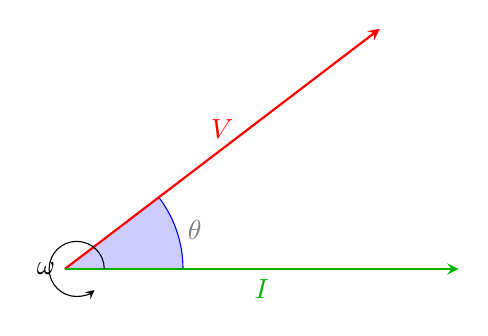
\begin{tikzpicture}[>=stealth,scale=5]

\filldraw[fill=blue!20!white,draw=blue] (0,0) -- (0.3,0) arc (0:37.8:0.3); 
\draw[thick,color=red,->] (0,0) -- node[above] {$V$}(.8,0.61);
\draw[thick,color=black!30!green,->] (0,0) -- node[below] {$I$} (1,0);
\node[color=gray] at (0.33,0.1) {$\theta$};
\draw[draw=black,->] node[left]{$\omega$}(0.1,0) arc (0:310:0.07); 
\end{tikzpicture}\par
\end{centering}
(or accept sinusoids vs time sketch, providing phase relationship approximately correct)
\end{enumerate}
The factory is required to raise its power factor to 0.9. 
\begin{enumerate}[resume,label=\alph*)]

\item \lbrack\ 2 marks ]\ Explain what the factory  can do to achieve this, assuming the existing machinery is retained.\par
Add capacitive reactive load until $\cos\theta=0.9$
\item \lbrack\ 2 marks ]\ What is the new apparent power for the whole plant, once a power factor of 0.9 has been achieved?\par
$P_\mathrm{A}=\dfrac{P_\mathrm{R}}{\mathrm{pf}}=\dfrac{150}{0.9}=\SI{166.6}{\kVA}$
\item \lbrack\ 2 marks ]\ What is the current now drawn by the plant.\par
$I=\dfrac{P_\mathrm{A}}{V}=\dfrac{166.6}{4}=\SI{41.65}{\ampere}$
\item \lbrack\ 2 marks ]\ Explain why the utility company that supplies the power might have required that the power factor be raised.\par
The current required for the same useful power at the plant is reduced, hence reducing transmission losses, losses in the site transformer and the required spec. of this transformer.
\end{enumerate}

\bigskip
\paragraph{\textbf{Solutions to Question 2} \ }

A white painted space heating radiator contains water at \SI{80}{\celsius} and is made of steel \SI{2}{\milli\metre} thick. The surrounding air is at \SI{20}{\celsius}. The required rate of heat transfer is \SI{2}{\kilo\watt}

\begin{enumerate}[label=\alph*)]
\item \lbrack\ 3 marks ]\ Sketch the temperature distribution along a cross-section through the radiator wall from the bulk water to the bulk air
\begin{figure}[h]
\centering
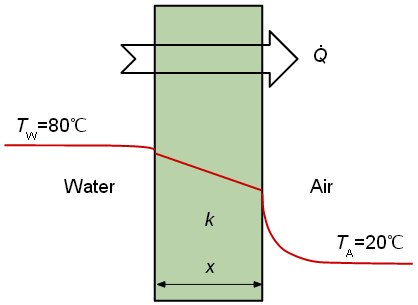
\includegraphics[width=0.5\textwidth]{./figures/RadiatorTprofile}
\end{figure}

\item \lbrack\ 4 marks ]\ Calculate $Q_\mathrm{C}$, the rate of heat transfer to the air by conduction and  convection, per square metre of radiator surface area.\par

$\Delta T=80-20=\SI{60}{K}$\par	
The overall resistance is the sum of the steel wall resistance and the steel-air surface resistance.

$R_{\rm T}=R_{\rm wall}+R_{\rm surface}=\dfrac{0.002}{50}+0.1=\SI{0.1}{\per\watt\kelvin\metre\squared}$\par	
Hence\par
$U=\dfrac{1}{R_{\rm T}}=\SI{10}{\watt\per\kelvin\per\metre\squared}$\par
so the heat transfer to the air by conduction and convection is given by

$Q_\mathrm{C}=U\Delta T=10\cdot 60=\SI{600}{\watt\per\metre\squared}$

\item \lbrack\ 3 marks ]\ Calculate $Q_\mathrm{R}$,  the rate of heat transfer to the air by radiation, per square metre of radiator surface area.
\begin{align*}
Q_\mathrm{R}&=\sigma\epsilon (T_1^4-T_2^4)\\
&=\SI{5.67e-8}{}\cdot\ 0.85\ \cdot (353.15^4-293.15^4)\\
&=\SI{393.7}{W}
\end{align*}
\item \lbrack\ 2 marks ]\ Calculate the required surface area of the radiator.\par
$A=\dfrac{2000}{600+393.7}=\SI{2.0}{\metre\squared}$
\item \lbrack\ 2 marks ]\ Why do you think it is a reasonable assumption to neglect the internal surface resistance?\par
Much higher density and thermal conductivity of water wrt air means that thermal transfer coefficient will be much lower
\end{enumerate}

You may assume that the external surface-air resistance is \SI{0.1} {\metre\squared\kelvin\per\watt} and that the internal surface resistance is negligible. The steel has thermal conductivity \SI{50}{\watt\per\kelvin\per\metre} and the white painted surface of the radiator has emissivity 0.85.

\bigskip
\paragraph{\textbf{Solutions to Question 3} \ }
Oil is to be heated from \SI{20}{\celsius} to \SI{50}{\celsius} using water entering a heat exchanger at \SI{80}{\celsius} and leaving at \SI{60}{\celsius}. A shell and tube in-line heat exchanger is to be used, in a counterflow arrangement. 
\begin{enumerate}[label=\alph*)]
\item \lbrack\ 3 marks ]\ Draw a sketch that shows the temperature distribution of the two fluids along the length of the heat exchanger.\\
\begin{figure}[h]
\centering
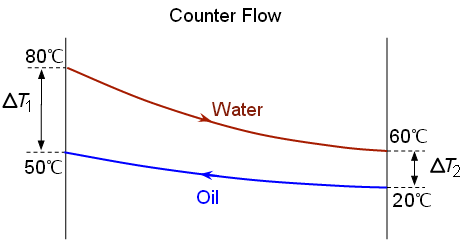
\includegraphics[width=0.5\textwidth]{./figures/CounterFlowHeatExchanger}
\end{figure}
\item \lbrack\ 2 marks ]\ Cite two advantages that the counterflow arrangement has over a parallel flow arrangement.\par
Mean temperature difference is greater so required surface area of contact is smaller; more constant temperature difference along length of heat exchanger, so thermal stress more even throughout.
\item \lbrack\ 3 marks ]\ What mass flow rate of water is required if heat is to be transferred at the rate \SI{2}{\kilo\watt}?
\begin{align*}
\dot Q&=\dot m c\Delta T\\
\mathrm{so}\\
\dot m &= \dfrac{\dot Q}{c\Delta T}=\dfrac{2}{4.2\cdot 20}=\SI{0.024}{\kg\per\second}
\end{align*}
\end{enumerate}
Specific heat capacity of water =\SI{4.2}{\kilo\joule\per\kg\per\kelvin}

\end{comment}

\end{document}

